\section{Summary of testing}
In the preceding chapter we defined and discussed aspects of the project relating to testing.
We defined two types of test: black-box, where you test the system without access to the code, and white-box, where the tester knows the details of how the software works.
Unit testing was our primary method of testing the system, and we used Mocha, Chai, Sinon and Nyc as test drivers.
We focused on testing conditional rendering and business logic in the front end, and having a high coverage percentage on controllers and middleware in the API.
We ended with a code coverage as seen on \autoref{fig:code-coverage}.
\begin{figure}[]
    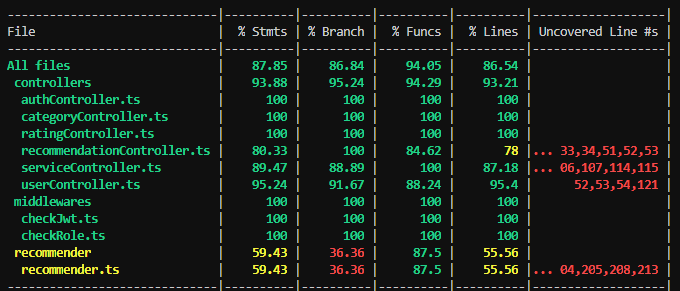
\includegraphics[width=\textwidth]{/codecoverage.png}
     \caption{Shows the coverage of our unit tests}
     \label{fig:code-coverage}
 \end{figure}
Integration testing was used to test external libraries, but did not deem it as important as unit testing.
To ensure correctness of the tests and quality of the code, we used formal reviews.
We did this by pairing up when doing reviews and using a CI.
We researched mutation testing, but ultimately did not end up applying it, due to lack of support for our language and test driver.
To evaluate the design of the system we made use of usability testing.
Based on our usability testing, we learned that while the overall design was intuitive, some icons could be misinterpreted, the way we select multiple options was not communicated clearly enough and there was a bug when trying to re-render the page that shows information.
